\begin{figure}[h!]
	\centering
	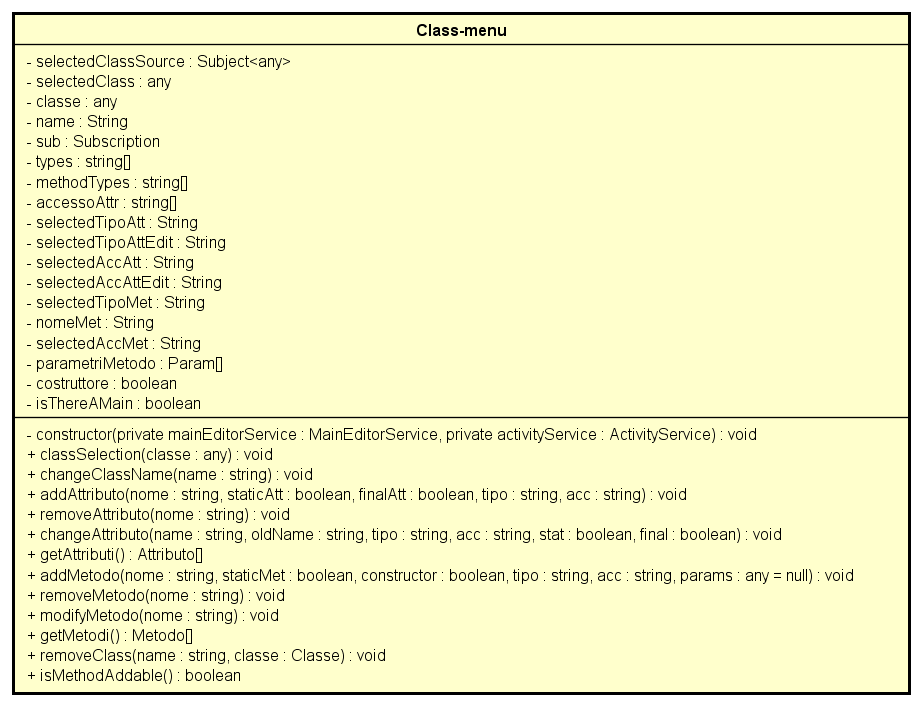
\includegraphics[scale=0.8]{res/sections/SpecificaFrontEnd/Services/Disegnetti/class-menu.png}
	\caption{Diagramma della classe Class-menu}
\end{figure}

\begin{itemize}
	\item \textbf{Descrizione:}\\
	
	\item \textbf{Utilizzo:}\\
	
	\item \textbf{Attributi:}
		\begin{itemize}
			\item \emph{-selectedClassSource: Subject<any>}\\
			Risorsa observable oggetto-classe
			\item \emph{-selectedClass: any}\\
			Stream observable oggetto-classe
			\item \emph{-classe: any}\\
			La classe correntemente selezionata nell'editor
			\item \emph{-name: string}\\
			Il nome della classe correntemente selezionata nell'editor
			\item \emph{-sub: Subscription}\\
			Subscription dell'oggetto observable che è la classe selezionata nell'editor
			\item \emph{-types: string[]}\\
			Array di tipi di dato primitivi
			\item \emph{-methodTypes: string[]}\\
			Array di tipi di dato primitivi per i tipi di ritorno dei metodi
			\item \emph{-accessoAttr: string[]}\\
			Array contenente le visibilità delle classi
			\item \emph{-selectedTipoAtt: string}\\
			Usato per memorizzare il tipo selezionato per il costruttore di un nuovo attributo
			\item \emph{-selectedTipoAttEdit: string}\\
			Usato per memorizzare il tipo selezionato per editare l'attributo
			\item \emph{-selectedAccAtt: String}\\
			Usato per memorizzare la visibilità selezionata per costruire un nuovo attributo
			\item \emph{-selectedAccAttEdit: String}\\
			Usato per memorizzare la visibilità selezionata per editare l'attributo
			\item \emph{-selectedTipoMet: String}\\
			Usato per memorizzare il tipo di ritorno selezionato per costruire un nuovo metodo
			\item \emph{-nomeMet: String}\\
			Usato per memorizzare il nome del nuovo metodo
			\item \emph{-selectedAccMet: String}\\
			Usato per selezionare la visibilità per costruire un nuovo metodo
			\item \emph{-parametriMetodo: Param[]}\\
			Usato per memorizzare un array di parametri per costruire un nuovo metodo
			\item \emph{-costruttore: boolean}\\
			Usato per memorizzare se il metodo è un costruttore
			\item \emph{-isThereAMain: boolean}\\
			Usato per memorizzare se è stato aggiunto il metodo main
		\end{itemize}
	\item \textbf{Metodi:}
		\begin{itemize}
			\item \emph{-constructor(private mainEditorService: MainEditorService,
    private activityService: ActivityService)}\\
    		Crea un istanziazione di ClassMenuComponent e setta le proprietà classe e nome per subscription da classMenuService\\
    		\textbf{Parametri:}
    		\begin{itemize}
    			\item \emph{mainEditorService: MainEditorService}\\
    			Usato per creare una nuova istanziazione di ClassMenuService
    			\item \emph{activityService: ActivityService}\\
    			Usato per creare una nuova istanziazione di ClassMenuService
    		\end{itemize}
    		\item \emph{+classSelection(classe: any)}\\
    		Comandi messaggio del servizio\\
    		\textbf{Parametri:}
    		\begin{itemize}
    			\item \emph{classe: any}\\
    			Variabile usata per settare la classe selezionata
    		\end{itemize}
    		\item \emph{+changeClassName(name: string)}\\
    		Cambia il nome della classe selezionata\\
    		\textbf{Parametri:}
    		\begin{itemize}
    			\item \emph{name: string}\\
    			Nuovo nome della classe
    		\end{itemize}
    		\item \emph{+addAttributo(nome: string, staticAtt: boolean, finalAtt: boolean, tipo: string, acc: string)}\\
    		Aggiunge un nuovo attributo alla classe\\
    		\textbf{Parametri:}
    		\begin{itemize}
    			\item \emph{nome: string}\\
    			Nome dell'attributo
    			\item \emph{staticAtt: boolean}\\
    			True se l'attributo è static
    			\item \emph{finalAtt: boolean}\\
    			True se l'attributo è final
    			\item \emph{tipo: string}\\
    			Tipo dell'attributo
    			\item \emph{acc: string}\\
    			Visibilità dell'attributo
    		\end{itemize}
    		\item \emph{+removeAttributo(nome: string)}\\
    		Rimuove un attributo dalla classe selezionata\\
    		\textbf{Parametri:}
    		\begin{itemize}
    			\item \emph{nome: string}\\
    			Nome dell'attributo da rimuovere
    		\end{itemize}
    		\item \emph{+changeAttributo(name: string, oldName: string, tipo: string, acc: string , stat: boolean, final: boolean)}\\
    		Modifica le proprietà di un attributo della classe selezionata\\
    		\textbf{Parametri:}
    		\begin{itemize}
    			\item \emph{name: string}\\
    			Nuovo nome dell'attributo
    			\item \emph{oldName: string}\\
    			Vecchio nome dell'attribuo
    			\item \emph{tipo: string}\\
    			Tipo dell'attributo
    			\item \emph{acc: string}\\
    			Tipo di visibilità
    			\item \emph{stat: boolean}\\
    			True se è marcato static
    			\item \emph{final: boolean}\\
    			True se è marcato final
    		\end{itemize}
    		\item \emph{+getAttributi()}\\
    		Ritorna la lista degli attributi di una classe
    		\item \emph{+addMetodo(nome: string, staticMet: boolean, constructor: boolean, tipo: string, acc: string, params: any = null)}\\
    		Aggiunge un nuovo metodo alla classe selezionata\\
    		\textbf{Parametri:}
    		\begin{itemize}
    			\item \emph{nome: string}\\
    			Nome del metodo
    			\item \emph{staticMet: boolean}\\
    			True se è marcato static
    			\item \emph{constructor: boolean}\\
    			True se è un costruttore
    			\item \emph{tipo: string}\\
    			Tipo del metodo
    			\item \emph{acc: string}\\
    			Visibilità del metodo
    			\item \emph{params: any = null}\\
    			Lista di parametri del metodo
    		\end{itemize}
    		\item \emph{+removeMetodo(nome: string)}\\
    		Rimuove un metodo dalla classe selezionata\\
    		\textbf{Parametri:}
    		\begin{itemize}
    			\item \emph{nome: string}\\
    			Nome del metodo da rimuovere
    		\end{itemize}
    		\item \emph{+modifyMetodo(nome: string)}\\
    		Setta la modalità activity nell'editor per editare il metodo della classe selezionata\\
    		\textbf{Parametri:}
    		\begin{itemize}
    			\item \emph{nome: string}\\
    			Nome del metodo da editare
    		\end{itemize}
    		\item \emph{+getMetodi()}\\
    		Ritorna la lista dei metodi di una classe
    		\item \emph{+removeClass(name: string, classe: Classe)}\\
    		Rimuove la classe selezionata\\
    		\textbf{Parametri:}
    		\begin{itemize}
    			\item \emph{name: string}\\
    			Nome della classe
    			\item \emph{classe: Classe}\\
    			Tipo della classe
    		\end{itemize}
    		\item \emph{+isMethodAddable()}\\
    		Ritorna true se il metodo è aggiungibile dalla logica
		\end{itemize}
\end{itemize}